% Este archivo es parte de la memoria del proyecto fin de carrera
% de Manuel López Urbina. Protegida bajo la licencia GFDL.
% Para más información, la licencia completa viene incluida en el
% fichero fdl-1.3.tex

% Copyright (C) 2012 Manuel López Urbina

\chapter{Interfaz gráfica}
\label{chap:interfaz-gráfica}

\section {Elementos de la interfaz gráfica}

Se consideró antes de comenzar el desarrollo de la interfaz gráfica, una serie de elementos mínimos imprescindibles que dicha interfaz debería incorporar.\\

Dada las características del proyecto, era necesario proporcionar a la aplicación de una interfaz gráfica sencilla pero a la vez funcional teniendo como principal objetivo ofrecer al usuario, tras una visión rápida, la localización de los diferentes elementos para control del vehículo y deducir su funcionamiento.\\

En este punto se realiza una descripción de los diferentes elementos presentes en la interfaz gráfica, la cual se compone de dos ventanas, una ventana principal donde se visualiza el estado del vehículo permitiendo su control y una segunda ventana para proporcionar información o ayuda al usuario.\\

Los elementos incorporados en la ventana principal son los siguientes:

\begin{itemize}

\item Panel para el visionado de las imágenes captadas por la cámara.

\item Conjunto de botones para manejo del vehículo, con imágenes representativas de su acción.

\item Panel para el visionado de resultados donde se mostrarán aquellas señales de tráfico detectadas.

\item Información acerca del detector de distancias.

\end{itemize}

La figura \ref{fig:ventana-principal} muestra una imagen de la ventana principal de la aplicación:\\

\begin{figure}[H]
  \begin{center}
    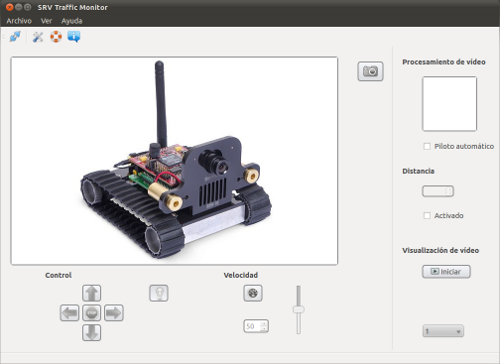
\includegraphics[scale=0.5]{ventana-principal.png}
  \end{center}
  \caption{Vista de la ventana principal.}
  \label{fig:ventana-principal}
\end{figure}

En el manual de usuario se encuentra disponible toda la información acerca del modo de utilización de la interfaz gráfica. Ver sección \ref{chap:manual-usuario}.\\

La ventana secundaria proporcionara información al usuario acerca de los controles del teclado, del gamepad, y otras informaciones de uso como dirección ip del vehículo. Esta ventana ha sido desarrollada con la intención, en mejoras futuras, permitir que dichos parámetros sean configurables.\\

La figura \ref{fig:ventana-información} muestra una imagen de la ventana de información:

\begin{figure}[H]
  \begin{center}
    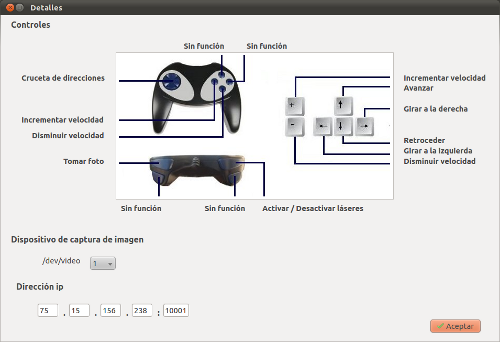
\includegraphics[scale=0.5]{ventana-controles.png}
  \end{center}
  \caption{Vista de la ventana de información.}
  \label{fig:ventana-información}
\end{figure}.


%En cuanto a aspectos técnicos,

%Dado que la imagen de entrada es obtenida mediante el uso de la función proporcionada por OpenCV, ésta se encuentra almacenada el la estructura de datos de la mencionada biblioteca, por tanto, resulta necesario definir un método de conversión del tipo de imagen IplImage de OpenCV al QImage propio de Qt con el fin de mostrar en la interfaz lo que se visualiza a través de la cámara en todo momento.

%Para la elaboración de la interfaz gráfica se ha empleado el IDE QtCreator haciendo uso de la biblioteca Qt, todo ello bajo un entorno GNU Linux.





